\documentclass[eng,openany]{mgr}
\usepackage{listings}
\usepackage[english]{babel}
\usepackage{graphicx}
\usepackage{hyperref}
\usepackage{tabularx,colortbl} 
\usepackage{rotating}
\usepackage{amsmath}
\usepackage[utf8]{inputenc} 
\setlength\parindent{24pt}
\usepackage[parfill]{parskip}
\usepackage[table,kernelfbox,hyperref]{xcolor}
\usepackage{fancyhdr}
\usepackage{gauss}
%\usepackage[colorinlistoftodos]{todonotes}

\hypersetup{colorlinks=true}
\hypersetup{xurlbordercolor=red!70!black}
\hypersetup{xlinkbordercolor=blue!70!black}
\hypersetup{linkcolor=blue!60!black}
\hypersetup{urlcolor=red!50!black}
\hypersetup{citecolor=green!30!black}
\rfoot{Page \thepage}
\renewcommand\lstlistlistingname{List of Listings}
\newcommand{\linia}{\rule{\linewidth}{0.4mm}}

\definecolor{listlightgray}{gray}{0.97}

\newcommand{\lstsetmylst} {
\lstset{frame = tb,
breaklines=true,
framerule = 0.1pt,
float,
fontadjust,
backgroundcolor={\color{listlightgray}},
basicstyle = {\ttfamily\footnotesize},
identifierstyle = {\ttfamily},
stringstyle = {\ttfamily},
showstringspaces = false,
showtabs = false,
numbers = left,
numbersep = 6pt,
tabsize = 4,
language=C,
floatplacement=!h
}
}

\newcommand{\lstsetatc} {
\lstset{frame = tb,
breaklines=true,
framerule = 0.25pt,
float,
fontadjust,
backgroundcolor={\color{listlightgray}},
basicstyle = {\ttfamily\footnotesize},
keywordstyle = {\ttfamily\color{listkeyword}\textbf},
identifierstyle = {\ttfamily},
commentstyle = {\ttfamily\color{listcomment}\textit},
stringstyle = {\ttfamily},
showstringspaces = false,
showtabs = false,
numbers = left,
numbersep = 6pt,
numberstyle={\ttfamily\color{listnumbers}},
tabsize = 4,
language=C,
floatplacement=!h
}
}

\newcommand{\lstsetatbashnum} {
\lstset{frame = tb,
breaklines=true,
framerule = 0.25pt,
aboveskip=2ex,
float,
fontadjust,
backgroundcolor={\color{listlightgray}},
basicstyle = {\ttfamily\footnotesize},
keywordstyle = {\ttfamily\color{listkeyword}\textbf},
identifierstyle = {\ttfamily},
commentstyle = {\ttfamily\color{listcomment}\textit},
stringstyle = {\ttfamily},
showstringspaces = false,
showtabs = false,
numbers = left,
numbersep = 6pt,
numberstyle={\ttfamily\color{listnumbers}},
tabsize = 4,
language=bash,
floatplacement=!h
}
}
\lstsetmylst
\author{Jaroslaw M. Szumega}
\title{}
\engtitle{}
\supervisor{Rafal Zdunek, D.Sc, K-4/W4}
\field{Electronics}
\specialisation{Advanced Applied Electronics}
\date{25.04.2017}
\begin{document}
\selectlanguage{english}
\maketitle
\tableofcontents
\chapter{Solution to the given problems}
\begin{figure}[h]
\centering
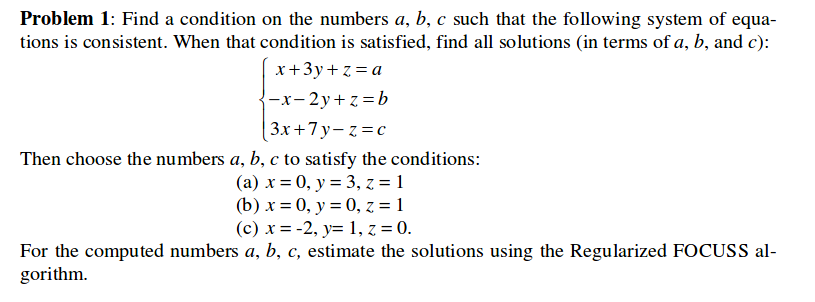
\includegraphics[width=0.8\linewidth]{screenshot001}
\label{fig:screenshot001}
\end{figure}
To find the mentioned condition, the RREF (Row Reduced Echelon Form) will be used.


\[
\begin{bmatrix}
1 & 3 & 1  &| & a\\
-1 & -2 & 1&| & b\\
3 & 7 & -1 &| & c
\end{bmatrix}
-- RREF -->
\begin{bmatrix}
1 & 0 & -5  &| & -2a -3b\\
0 & 1 & 2&| & a + b\\
0 & 0 & 0 &| & -a + 2b + c
\end{bmatrix}
\]

Regarding to the obtained result, the system is  consistent only when the condition is fulfilled:
\begin{center}
$-a + 2b + c = 0$
\end{center}

The solution interpreted from the RREF 
matrix is:
\begin{align}
x_1 &= -2a - 3b\nonumber\\
x_2 &=   a + b - 2x_3\nonumber\\
x_3 &= free variable \nonumber
\end{align}

In above mentioned solution, the $x_3$ is a free variable, which means that it is not bounded to any specific value. We can interpret is as a solution's parameter.\\
To estimate it, we should have some kind of knowledge that will bound it even before the solving process.
\lstset{basicstyle=\scriptsize}
\begin{lstlisting}
 b =
 10
 -5
 20
 
 x_calcA =
 0.00000
 3.00000
 1.00000
 
 Elapsed time is 0.022619 seconds.
 
 b_calculatedA =
 10.0000
 -5.0000
 20.0000
 
solution_error =    4.4052e-07
residual_error =    6.9201e-07
 
 b =
 1
 1
 -1
 
 x_calcB =
 0.00000
 0.00000
 1.00000
 
 Elapsed time is 0.00672603 seconds.
 
 b_calculatedB =
 1.00000
 1.00000
 -1.00000
 
solution_error =    3.3345e-07
residual_error =    5.7755e-07
 
 b =
 1
 0
 1
 
 x_calcC =
 0.00000
 0.20000
 0.40000
 
 Elapsed time is 0.00638103 seconds.
 
 b_calculatedC =
 1.0000e+00
 -5.2708e-07
 1.0000e+00
 
solution_error =    2.1909
residual_error =    1.1900e-06
\end{lstlisting}


The calculated solution for cases 'a' and 'b' are corresponding to the data pointed out for them. For case 'c' however, the calculated solution differs quite much.\\
The 'c' solution is not exact, but the estimate errors are rather small. Knowing the system purpose, it would be possible to assess if the model is usefull. \newpage

\begin{figure}[h]
\centering
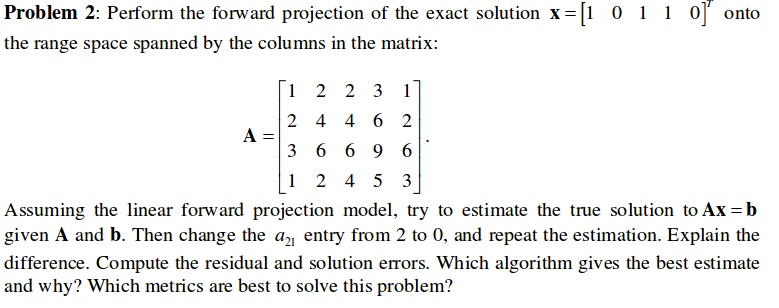
\includegraphics[width=0.7\linewidth]{screenshot002}
\label{fig:screenshot002}
\end{figure}

For the selected problem the multiple algorithms were used for calculations. Both scenarios, indicated in the introduction were taken under consideration.
\\
$a_{21} = 2$
\begin{lstlisting}
Regularized focuss
Elapsed time is 0.00539589 seconds.

x_transposed =
0.00000   1.00000   2.00000   0.00000   0.00000

solution_error =  2.0000
residual_error =    2.3452e-07



MFocuss
Elapsed time is 0.00734401 seconds.

x_transposed =
0.00000   0.00000   0.00000   1.00000   0.00000

solution_error =  1.4142
residual_error =  12.288



Tikhonov
Elapsed time is 0.000128984 seconds.

x_transposed =
0.193639   0.387279   0.877795   1.071435   0.038132

solution_error =  0.90647
residual_error =  0.084187



QR LS
(warning during algorithms operation: matrix singular to machine precision)
Elapsed time is 0.000256062 seconds.

x_transposed =
-0.660375   0.894607   0.894607   1.050346  -0.069089

solution_error =  1.8909
residual_error =  0.32342



SVD LS
Elapsed time is 0.000138998 seconds.

x_transposed =
1.8182e-01   3.6364e-01   9.0909e-01   1.0909e+00   2.3870e-15

solution_error =  0.90453
residual_error =    1.5511e-14
\end{lstlisting}
\newpage
$a_{21} = 0$
\begin{lstlisting}
2. Regularized focuss
Elapsed time is 0.0136371 seconds.

ans =
1.00000  -0.50000   0.00000   2.00000   0.00000

solution_error =  1.5000
residual_error =    1.6575e-06



2. MFocuss
Elapsed time is 0.012074 seconds.

ans =
1.00000   0.00000   1.00000   1.00000   0.00000

solution_error =    9.5263e-10
residual_error =    1.3265e-08



2. Tikhonov
Elapsed time is 0.000120878 seconds.

ans =
0.764147   0.092481   0.899610   0.945850   0.214162

solution_error =  0.35079
residual_error =  0.23123



2. QR LS
Elapsed time is 0.000169039 seconds.

ans =
1.0000e+00  -6.6613e-16   1.0000e+00   1.0000e+00  -1.8328e-15

solution_error =    3.4265e-15
residual_error =    4.6998e-15



2. SVD LS
Elapsed time is 0.000123024 seconds.

ans =
1.0000e+00   7.7716e-16   1.0000e+00   1.0000e+00  -2.6645e-15

solution_error =    5.2791e-15
residual_error =    6.9369e-15
\end{lstlisting}

In the first case, the results did not correspond to the original x vector. In second scenario, the algorithms were able to  calculate precise or almost exact value of x.
It is mainly due to the condition number of both matrices:
\begin{itemize}
	\item $a_{21} = 2 $: cond(A) ~= 2e16
	\item $a_{21} = 0 $: cond(A) ~= 28
\end{itemize}

In the second case (which gave better result), the algorithms that calculated the most optimal solution were MFOCUSS and variations of LS for under-determined systems (QR, SVD options). \newpage
\begin{figure}[h]
\centering
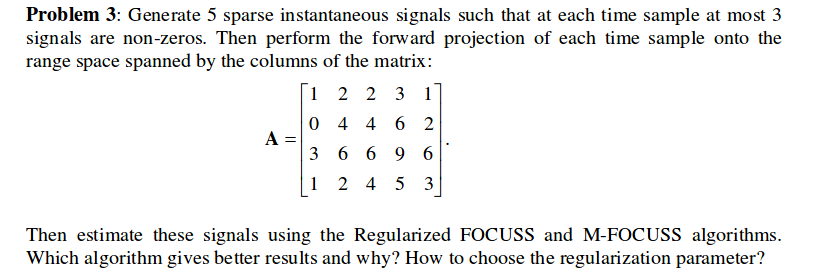
\includegraphics[width=0.7\linewidth]{screenshot003}
\label{fig:screenshot003}
\end{figure}
To start, the 5 signals had to be generated. The Octave code shown below did this, the comments are attached.
\begin{lstlisting}
#generation of five signals, now 100 samples each
x = randn(5,100);

#convert to "discrete", it will help with estimating the "non-zeros" condition
x(x < 0) = 0;
x(x > 0) = 1;

#sum to find when condition "at most 3 non zeros at the time" is exceeded
E = sum(x,1);
n = find(E>3);

#and wipe when more than 3 are non-zeros
x(:,n) = [];
\end{lstlisting}
At this point, at least quite a few signals are generated according to the condition indicated in the task. However, we only need 5 of them.

The results are presented below:
\begin{lstlisting}
Signal no. 1
0   0   1   1   0

Focuss
xFOCUSS_transposed =
0.00000   0.00000   1.00277   1.01478   0.00000

solution_error =  0.015034
residual_error =  0.20503


MFocuss
xMFOCUSS_transposed =
0.00000   0.00000   0.99895   1.00187   0.00000

solution_error =  0.0021402
residual_error =  0.014051


Signal no. 2
1   0   1   0   1

Focuss
xFOCUSS_transposed =
0.99968   0.00000   1.00127   0.00000   1.00182

solution_error =  0.0022456
residual_error =  0.022535

MFocuss
xMFOCUSS_transposed =
1.00048   0.00000   1.00146   0.00000   1.00190

solution_error =  0.0024394
residual_error =  0.027004



Signal no. 3
0   1   0   0   0

Focuss
xFOCUSS_transposed =
0.00000   0.99784   0.00000   0.00000   0.00000

solution_error =  0.0021606
residual_error =  0.016736

MFocuss
xMFOCUSS_transposed =
0.00000   0.99833   0.00000   0.00000   0.00000

solution_error =  0.0016659
residual_error =  0.012904


Signal no. 4
0   0   1   0   0

Focuss
xFOCUSS_transposed =
0.00000   0.00000   1.00224   0.00000   0.00000

solution_error =  0.0022401
residual_error =  0.019007

MFocuss
xMFOCUSS_transposed =
0.00000   0.00000   0.99708   0.00000   0.00000

solution_error =  0.0029241
residual_error =  0.024811


Signal no. 5
1   1   0   0   1

Focuss
xFOCUSS_transposed =
1.00025   0.99820   0.00000   0.00000   0.99932

solution_error =  0.0019382
residual_error =  0.017824

MFocuss
xMFOCUSS_transposed =
1.00014   1.00462   0.00000   0.00000   1.00146

solution_error =  0.0048473
residual_error =  0.046094
\end{lstlisting}

The signals were estimated using regularization matrix $L = I (identity)$. \\Comparing both methods for each single case, there is no any spectacular difference between obtained solutions. Both of the errors are quite small in their value and solution is fairly estimated.
\newpage
\begin{figure}[h]
\centering
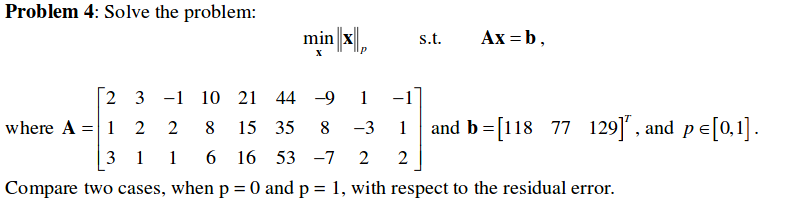
\includegraphics[width=0.7\linewidth]{screenshot004}
\label{fig:screenshot004}
\end{figure}
The tasks goal is to compare cases with parameter p = 0 and p = 1, which clearly indicates using of Focuss-family algorithms.\\
For the calculation below the parameter $\lambda = 1e-8$ was fixed and used during the computations.

\begin{lstlisting}
A =

2    3   -1   10   21   44   -9    1   -1
1    2    2    8   15   35    8   -3    1
3    1    1    6   16   53   -7    2    2

b =

118
77
129

x_exact =
0.0191812   0.0174549   0.0045213   0.0704225   0.1561079   0.4034636  -0.0369650   0.0039733   0.0059462

x_focuss0 =
0.00000   0.00000   0.00000   0.00000   1.00000   2.00000  -1.00000   0.00000   0.00000

x_focuss1 =
2.6276e-140    8.8686e-69   -6.9865e-63    1.9074e-30    1.0000e+00    2.0000e+00   -1.0000e+00    3.0741e-87   -7.6512e-62

x_mfocuss0 =
0.00000   0.00000   0.00000   0.00000   1.00000   1.00000  -1.00000   0.00000   0.00000

x_mfocuss1 =
0.00000   0.00000   0.00000   0.00000   1.00000   1.00000  -1.00000   0.00000   0.00000



Solution Errors:

e_focuss0 =    1.5787e-09
e_focuss1 =    1.2990e-09
e_mfocuss0 =  77.266
e_mfocuss1 =  77.266
\end{lstlisting}
While the solutions itself may not be very meaningful, the errors values usually are.\\
In this particular case, the computations vere conducted a few times, mostly because the MFOCUSS algorithm result were very similar in both cases of parameter p value.

To sum up: the results again were not exact, but very well approximated. The residual erors for FOCUSS algorithm were small. In case of MFOCUSS quite larger (in case of any mistake in Octave code or algorithm's coded, there were multiple checks, but nothing incorrect was found).
\newpage


\begin{figure}[h]
\centering
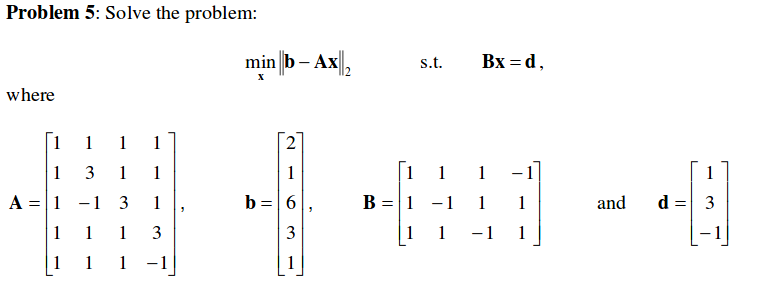
\includegraphics[width=0.7\linewidth]{screenshot005}
\label{fig:screenshot005}
\end{figure}

To solve above-mentioned problem, the LS algorithm with equality constraints was chosen to be compared with built-in Octave function \textbf{lsqlin}.

\begin{lstlisting}
LS algorithm with equality constraints:

x =
0.75000
-0.75000
1.25000
0.25000

Elapsed time is 0.017941 seconds.
e_Ax =    1.7092e-15
e_Bd =    6.6613e-16



Lsqlin algoritm:

x_octave =
0.50000
-0.50000
1.50000
0.50000

Elapsed time is 0.00419497 seconds.
e_OctaveAx =    1.7092e-15
e_OctaveBd =    6.6613e-16
\end{lstlisting}

What can be noticed is that in both cases the residual errors (because these were calculated) are the same.\\
The execution time seems to be better in case of built in function. And in fact there is not much more to comment.


\newpage
\begin{figure}[h]
\centering
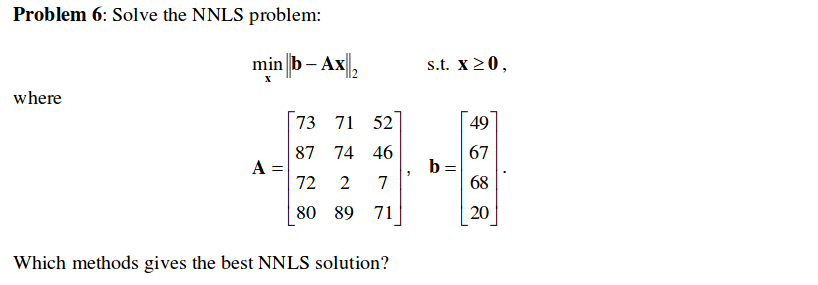
\includegraphics[width=0.7\linewidth]{screenshot006}
\label{fig:screenshot006}
\end{figure}
In task 6, the NNLS algorithm (interior point version) was coded and used. For the task, the hardcoded limit of 1000 iterations was set.
\\To have a comparison, also the built-in \textbf{lsqnonneg} function was used for computations.

\begin{lstlisting}
Elapsed time is 0.00615311 seconds.
x_nnls =
3.3062e-01
4.1365e-05
7.2307e-01

error_nnls =  71.122



Elapsed time is 0.00321317 seconds.
x_octave =
0.64954
0.00000
0.00000

error_octave =  39.813
\end{lstlisting}
The performance in case of error value was much better in Octave's lsqnonneg function. The same is for the computation time.
\newpage
\begin{figure}[h]
\centering
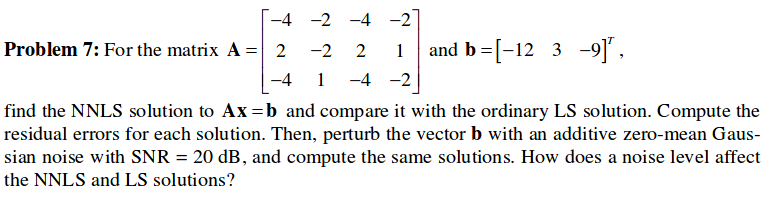
\includegraphics[width=0.7\linewidth]{screenshot007}
\label{fig:screenshot007}
\end{figure}

\begin{lstlisting}
x_nnls =
-0.053757
1.041759
1.702508
1.616885

e_nnls =  0.28882


General Crossvalidation cannot be used due to "machine's precision" error.

x_QR =
2.2204e-16
1.0000e+00
2.0000e+00
1.0000e+00

Elapsed time is 0.000808954 seconds.
e_qr =    2.5121e-15

x_SVD =
-8.8818e-16
1.0000e+00
2.0000e+00
1.0000e+00

Elapsed time is 0.000778913 seconds.
e_svd =    8.9811e-15


b perturbed by noise

x_nnls =
5.4629e-01
7.1885e-01
8.6128e-05
4.4108e+00

e_nnls =  3.1961

x_QR =
0.023284
1.004230
2.006133
1.003067

Elapsed time is 0.000202894 seconds.
e_qr =    2.6645e-15

x_SVD =
0.023284
1.004230
2.006133
1.003067

Elapsed time is 0.000172138 seconds.
e_svd =    1.0986e-14
\end{lstlisting}

According to the result -- the noise introduces a change in solution estimation, however, that change is larger in case of computing NNLS solution. The classical LS (using svd, qr) were not affected that much.
\newpage
\begin{figure}[h]
\centering
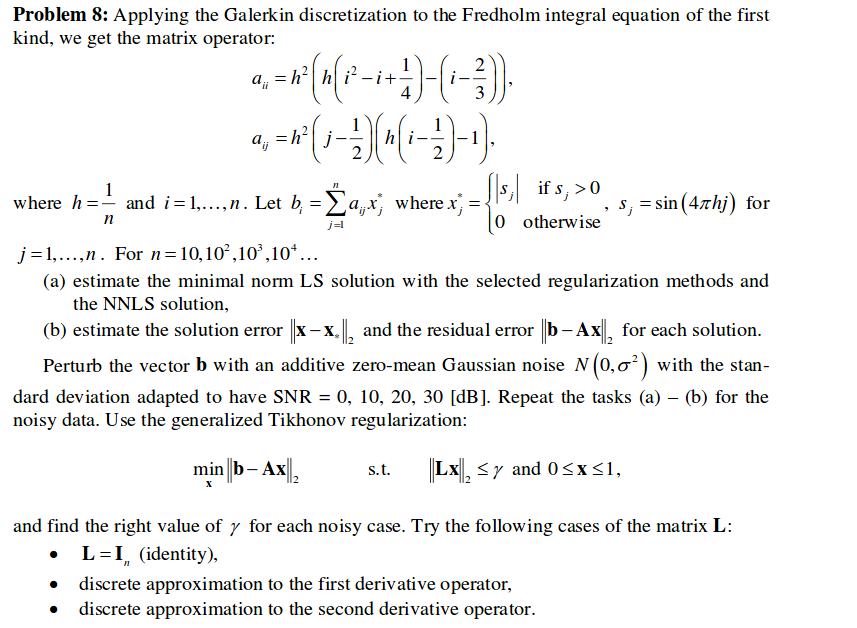
\includegraphics[width=0.7\linewidth]{screenshot008}
\label{fig:screenshot008}
\end{figure}
To filfill Task8, the function to initialize the testing environment (meaningful name of the function -- \textbf{galerkin\_init}) was prepared.\\
All the calculations were dune using regularization matrix\\ $L = I (identity)$, as well as the first derivative.\\

Due to the problem size and solution space (the following powers of 10), only the numerical results of solution and residual errors will be shown.

\begin{figure}[h]
\centering
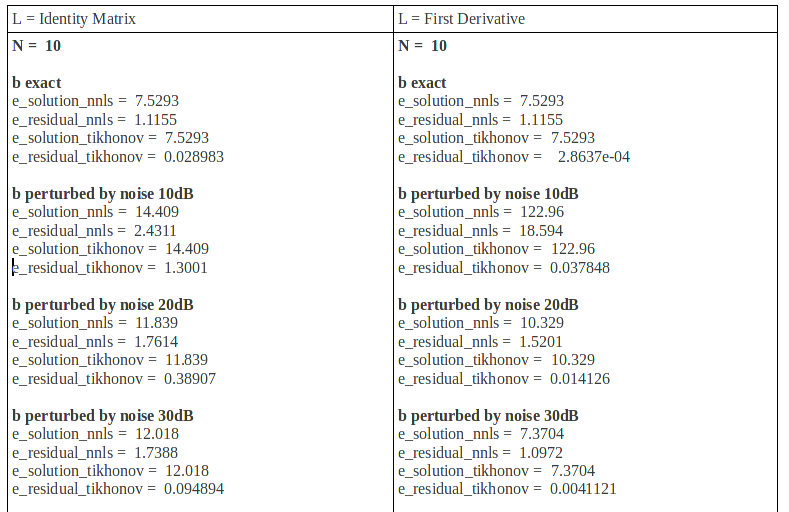
\includegraphics[width=0.7\linewidth]{screenshot009}
\caption{Computations for n = 10}
\label{fig:screenshot009}
\end{figure}

\begin{figure}[h]
\centering
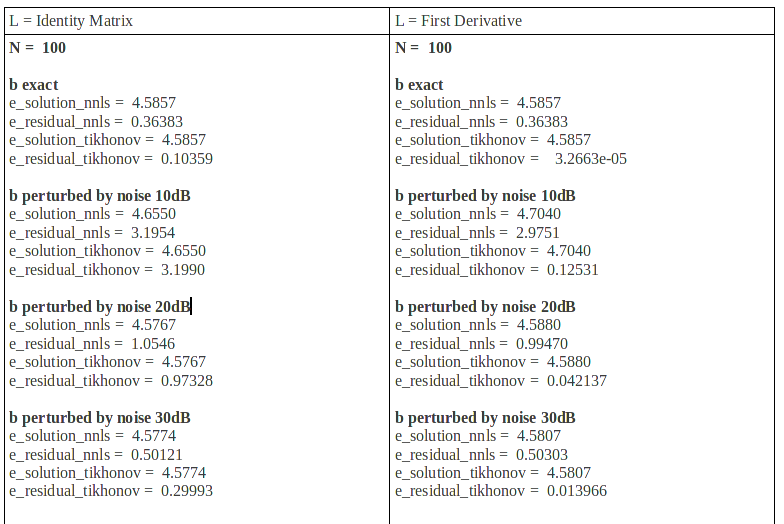
\includegraphics[width=0.7\linewidth]{screenshot010}
\caption{Computations for n = 100}
\label{fig:screenshot010}
\end{figure}

\begin{figure}[h]
\centering
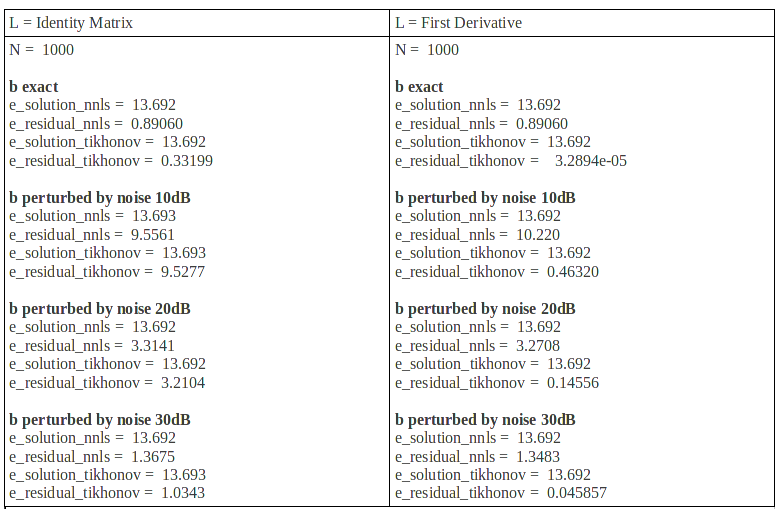
\includegraphics[width=0.7\linewidth]{screenshot011}
\caption{Computations for n = 1000}
\label{fig:screenshot011}
\end{figure}
By looking at the results, the interesting facts can be noticed.\\
1. In case of using NNLS algorithm, there is no difference between using Identity Matrix or First Derivative operator as a regularization matrix. The Solution and Residual errors are quite similar.\\
2. The very interesting case is for N = 10 and L = First derivative.\\The error calculated from both NNLS and Tikhonov solutions suddenly increased.\\
3. The Tikhonov regularization performed better in measure of residual error of the solution. It had even better result, when the regularization was First Derivative operator.
\chapter{Algorithms code}
Algorithm \space 1 -- FOCUSS algorithm.\\
\begin{lstlisting}
function [x] = focuss(A,b,p,lambda, regul)

[m,n] = size(A);

x = rand(n,1);

#when reg = I, then we have generalized focuss
if(regul == 1)
regul = eye(m);
endif

for k = 1:100
W=diag(abs(x)).^(1-p/2);
W2 = W.*W;
x=W2*A'*inv(A*W2*A'+lambda*regul)*b;
endfor

endfunction

\end{lstlisting}
Algorithm \space 2 -- MFOCUSS\\
\begin{lstlisting}
function [x] = mfocuss(A,b,p,lambda)

[m,n] = size(A);
[o,p] = size(b);

x = ones(n,1);
I = eye(m);

for k = 1:100
%  norm of each row
w = sqrt(sum(abs(x).^2,2));
W=diag(w.^(1-p/2));

A = A * W;
Q = A'*inv(A*A'+lambda*I)*b;

x=W*Q;

endfor
endfunction

\end{lstlisting}

\newpage
Algorithm \space 3 -- LS by QR for underdetermined problems.\\
\begin{lstlisting}
function [x] = qrLS_underdetermined(A,b) 

[m,n] = size(A); 
[Q, R] = qr(A'); 

z = inv(R(1:m,1:m)')*b;
x = Q(:,1:m)*z;

endfunction

\end{lstlisting}

Algorithm \space 4 -- The LS solution by SVD for underdetermined problems.\\

\begin{lstlisting}
function [x] = svdLS_underdetermined(A,b) 

[m,n] = size(A); 

[u,s,v] = svd(A); 
v = v';

x = (s*v) \ (u'*b);
endfunction
\end{lstlisting}
Algorithm \space 5 -- The LS by equality constraints (nullspace)\\
\begin{lstlisting}
function [x] = equalityLS(A,b,C,d)

#according to
# https://stanford.edu/class/ee103/lectures/constrained-least-squares/constrained-least-squares_slides.pdf
# http://www.seas.ucla.edu/~vandenbe/133A/lectures/cls.pdf

x_exact = pseudoinverse(C)*d;

C_z = C';
d_z = A'*b - A'*A;;

z = pseudoinverse(C_z)*d_z;

if(isempty(z) == false)
x = x_exact;
endif


endfunction
\end{lstlisting}
\newpage
Algorithm \space 6 -- The interior-point NNLS\\
\begin{lstlisting}
function [x] = nnls(A,b, iterations)

[m,n] = size(A);

AtA = A'*A;
Atb = A'*b;

e = ones(n,1);

xk = ones(n,1);
yk = xk;

completed_iterations = 0;
for i = 1:iterations

completed_iterations = i;

Xk= diag(xk);
Yk= diag(yk);

mi = (xk' * yk) ./ (n^2);

#we have diagonal matrices, so we can spare some time
Xk_inv = diag(1./xk);
Xk_sqrt_inv = diag(1./sqrt(xk));

Yk_sqrt = diag(sqrt(yk));
Yk_sqrt_inv = diag(1./sqrt(yk));

#taking advantage that sqrt(a*b) = sqrt(a)*sqrt(b)
Fac1 = [A; Xk_sqrt_inv * Yk_sqrt]; 
Fac2 = [b - A * Xk * e; Xk_sqrt_inv * Yk_sqrt_inv * mi * e ];

uk = Fac1\Fac2;

vk = -Yk*e + Xk_inv *mi*e - Xk_inv *Yk*uk;

T1 = min(-xk(uk < 0) ./ uk(uk < 0));
T2 = min(-yk(vk < 0) ./ vk(vk < 0));

#exact book condition
theta = 0.99995 * max(T1,T2);

#if no further improvemeent, then... break
if isempty(theta)
break;
endif

xk = xk + theta*uk;
yk = yk + theta*vk;
end

x = xk;
completed_iterations;
endfunction
\end{lstlisting}
Algorithm \space 7 -- The General Crossvalidation\\
\begin{lstlisting}
function [x] = crossvalidation(A,b, mi)

C = inv(A'*A);

M = A' * A + (mi.^2).^C'*C;

x = inv(M)*A'*b;

endfunction
\end{lstlisting}
Algorithm \space 8 -- The Tikhonov regularization\\
\begin{lstlisting}
function [x] = tikhonovGen(A,b, alpha, L)

[m,n] = size(A);

if(L == 1)
	L = eye(n);
endif

x = inv(A' * A + alpha.*2*L'*L) * A' * b;

endfunction
\end{lstlisting}

Algorithm \space 9 -- Pseudoinverse\\
\begin{lstlisting}
function [x] = pseudoinverse(A)

[m,n] = size(A);
r = rank(A);
[u,s,v] = svdqr(A,20);

x = zeros(n,m);

for i = 1:r
x = x + inv(s(i,i)) *v(:,i)* u(:,i)';
endfor

endfunction
\end{lstlisting}
\begin{thebibliography}{8}
\addcontentsline{toc}{chapter}{Bibliography}
%\addcontentsline{toc}{section}{Literatura}
\bibitem{bjorck}
Björck, Åke. Numerical methods for least squares problems. Society for Industrial and Applied Mathematics, 1996.
\bibitem{meyer} 
Golub, G. H., \& Van Loan, C. F. (2012). Matrix computations (Vol. 3). JHU Press.
\bibitem{zdunek}
Zdunek R., Numerical Methods - lecture slides.
\end{thebibliography}

\end{document}

